\subsection{Description of the objective}

This step consists of the addition of the tracker. It will provide the client the list of chunks and the peers that own each chunk. The client will thus not have to fetch this information in a configuration file but still needs to know the IP address and port number of the tracker.

\subsection{Proposed solution}

The \texttt{tracker} class now implements the reading of the configuration file as the client did in step 1, in order to know the addresses, ports and chunks of the peers.

When a request is sent by the client to the tracker, all the file information is sent in a message. According to the content of this message, the list of chunks are placed in the adequate queues (only Alice, only Bob or owned by both). The file {\tt file.ini} is created and the follow-up is exactly the same as it was in step 1. The request to the tracker is sent using TCP to ensure that the correct IP and port will be received, as these are essentials to establish a connection with the peers.

\subsection{Sequence diagram}

The sequence diagram of the second step is shown in Figure \ref{fig:step2}.

The principle is very similar to the first step once the information of the file is received by the tracker. The connection with the tracker is established similarly to the connection with the peers, and the queues still offer the maximum transfer speed possible.

\begin{figure}
	\centering
	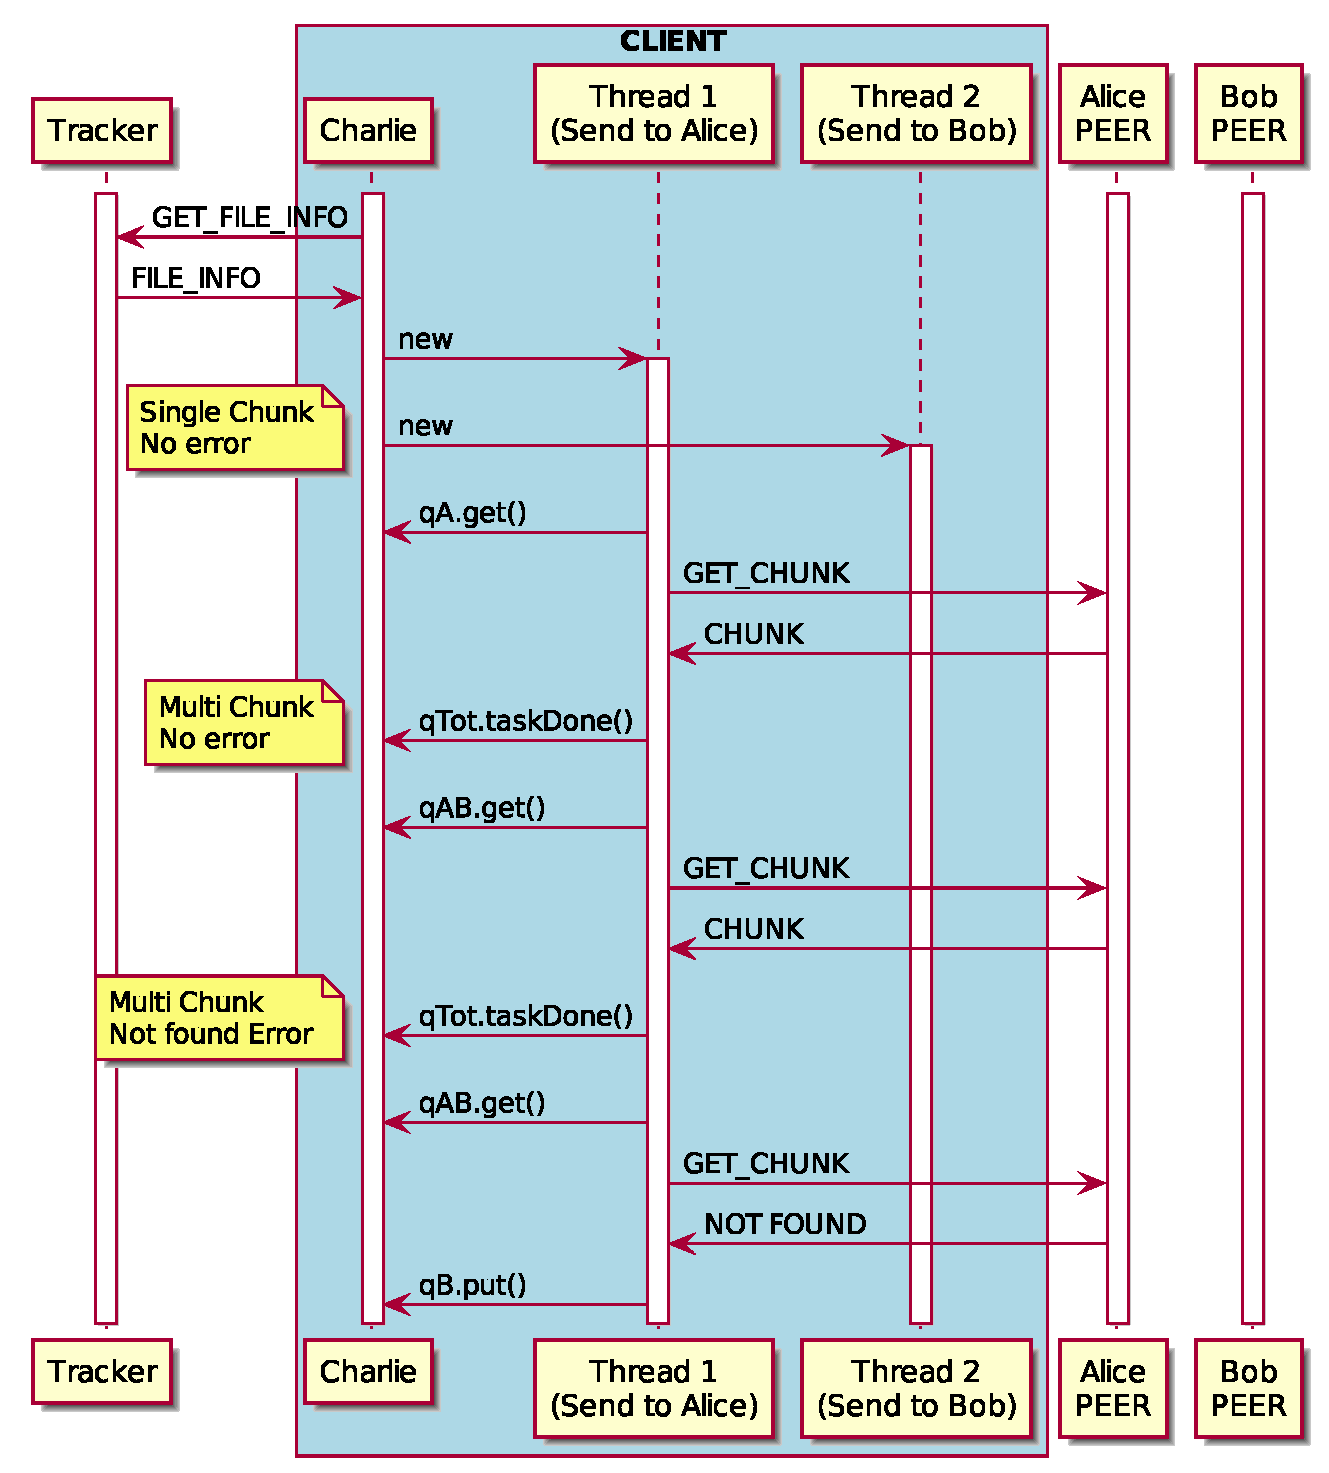
\includegraphics[width=\textwidth]{img/step2.eps}
	\caption{Sequence diagram of step 2}
	\label{fig:step2}
\end{figure}

\subsection{Bonus - contacting the lab tracker}

2 bonus points could be earned by contacting a tracker at the lab and downloading provided in chunks. As the IP address and the port number of this tracker were knowns, the code of the step 2 was able to contact the tracker, download the chunks and reconstruct the file (5 minutes of the \textit{Start Wars III} movie). It is to be noted that some chunks that were supposed to be owned by both peers were not, but the implementation with the queues allowed to handle it without any problem.


